\section{Erweiterung auf Graphen im zweidimensionalen euklidschen Raum}
\label{gcn_erweiterung}

Die Ansätze von~\citeauthor{Defferrard} aus Kapitel~\ref{spektraler_faltungsoperator} und~\citeauthor{gcn} aus Kapitel~\ref{graph_convolutional_networks} zeigen konkurrenzfähige Resultate auf einer Reihe von Datensätzen auf Graphen (\vgl{}~\cite{Defferrard, gcn}).
So erreicht das \gls{GCN} \zB{} in der teilweise-überwachten Knotenklassifizierung von Referenz-Graphen, \dhe{} einer Menge von Knoten, die Dokumente über eine Reihe von Bag-of-Words-Merkmalen repräsentieren und (ungerichtet) über dessen Referenzierungen miteinander verbunden sind, beachtliche Ergebnisse und schneidet in diesen sogar knapp besser ab als über die Tschebyschow-Approximation mit $K=2$ und $K=3$~\cite{gcn}.

Die spektrale Faltung auf Graphen entspricht einer Generalisierung der Faltung klassischer \glspl{CNN} auf zweidimensionalen Bildern~\cite{gcn_review}.
Es ist jedoch anzumerken, dass die spektrale Faltung im Gegensatz zur klassischen Faltung auf einem regulären Gitter insbesondere rotationsinvariant ist.
Das ist in der Regel für generelle Graphen keine Schwäche, schließlich kann den Knoten \bzw{} Kanten eines Graphen, kodiert als Adjazenzmatrix, keine Örtlichkeit \bzw{} Richtung (wie links, rechts, oben oder unten) zugeordnet werden.
Die Rotationsinvarianz kann folglich sowohl als Einschränkung oder Vorteil interpretiert werden, abhängig von dem Problem, welches man betrachtet~\cite{Defferrard}.

\begin{figure}[t]
\centering
\subfigure[Reguläres Gitter]{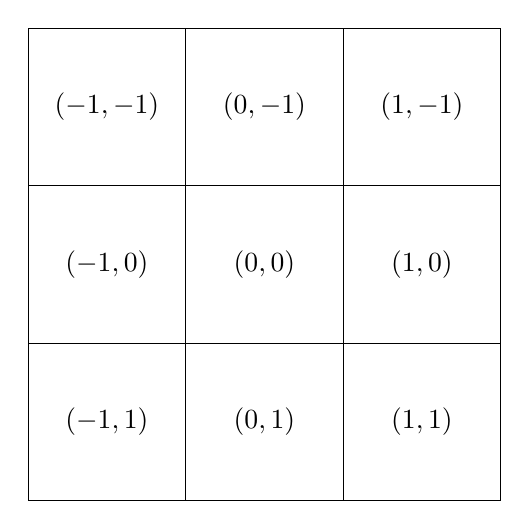
\begin{tikzpicture}
  \draw (-3, -3) rectangle (-1, -1) node[pos=0.5] {$\left(-1, 1\right)$};
  \draw (-1, -3) rectangle (1, -1)  node[pos=0.5] {$\left(0, 1\right)$};
  \draw (1, -3)  rectangle (3, -1)  node[pos=0.5] {$\left(1, 1\right)$};
  \draw (-3, -1) rectangle (-1, 1)  node[pos=0.5] {$\left(-1, 0\right)$};
  \draw (-1, -1) rectangle (1, 1)   node[pos=0.5] {$\left(0, 0\right)$};
  \draw (1, -1)  rectangle (3, 1)   node[pos=0.5] {$\left(1, 0\right)$};
  \draw (-3, 1)  rectangle (-1, 3)  node[pos=0.5] {$\left(-1, -1\right)$};
  \draw (-1, 1)  rectangle (1, 3)   node[pos=0.5] {$\left(0, -1\right)$};
  \draw (1, 1)   rectangle (3, 3)   node[pos=0.5] {$\left(1, -1\right)$};
\end{tikzpicture}
}
\hspace{1cm}
\subfigure[Graphrepräsentation]{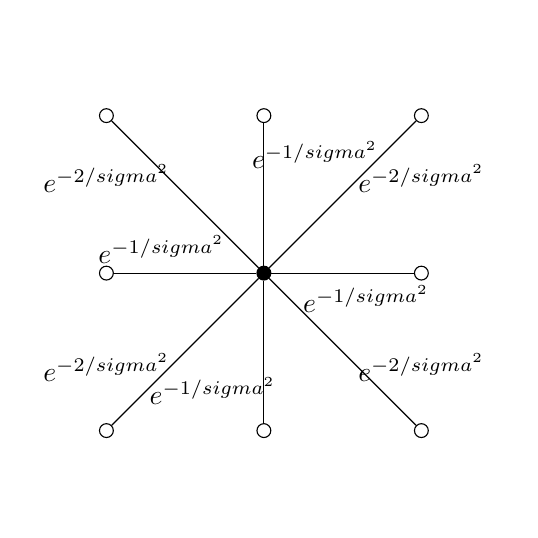
\begin{tikzpicture}
  \tikzstyle{node}=[circle,draw, minimum width=5pt, inner sep=0pt, fill=white]
  \tikzstyle{root}=[fill=black]
  \fill [white] (-3, -3) rectangle (3, 3) node {};  % Zentriere vertikal.

  \node[node] (00) at (-2, 2) {};
  \node[node] (01) at (0, 2) {};
  \node[node] (02) at (2, 2) {};
  \node[node] (10) at (-2, 0) {};
  \node[node, root] (11) at (0,0) {};
  \node[node] (12) at (2, 0) {};
  \node[node] (20) at (-2, -2) {};
  \node[node] (21) at (0, -2) {};
  \node[node] (22) at (2, -2) {};

  \path (10) edge node[shift={(-0.3, 0.3)}]  {$e^{-1/\gls{sigma}^2}$} (11);
  \path (11) edge node[shift={(0.3, -0.33)}]  {$e^{-1/\gls{sigma}^2}$} (12);
  \path (01) edge node[shift={(0.65, 0.5)}]   {$e^{-1/\gls{sigma}^2}$} (11);
  \path (11) edge node[shift={(-0.65, -0.5)}] {$e^{-1/\gls{sigma}^2}$} (21);
  \path (00) edge node[shift={(-1, 0.2)}]    {$e^{-2/\gls{sigma}^2}$} (11);
  \path (02) edge node[shift={(1, 0.2)}]     {$e^{-2/\gls{sigma}^2}$} (11);
  \path (11) edge node[shift={(1, -0.2)}]    {$e^{-2/\gls{sigma}^2}$} (22);
  \path (20) edge node[shift={(-1, -0.2)}]   {$e^{-2/\gls{sigma}^2}$} (11);
\end{tikzpicture}
}
  \caption[Graphrepräsentation eines regulären Gitters]{Illustration (a) eines $3 \times 3$ großen regulären Gitters zentriert um den Punkt $\left(0, 0\right)$ und (b) dessen lokale Nachbarschaft der entsprechenden Graphrepräsentation mit einer Konnektivität von $8$ bei horizontalen \bzw{} vertikalen Kantengewichten $\exp\left(-1/\gls{sigma}^2\right) \in \gls{R}$ und respektive $\exp\left(-2/\gls{sigma}^2\right) \in \gls{R}$ bei den Diagonalen.}
\label{fig:gcn_review}
\end{figure}


Im Kontext dieser Arbeit, dem Lernen auf Graphen im zweidimensionalen euklidschen Raum, bei denen Graphknoten eine eindeutige Position besitzen, ist die Rotationsinvarianz weitestgehend unerwünscht.
Das kann leicht verifiziert werden, indem wir den Filter des \glspl{GCN} auf einer Graphrepräsentation eines Gitters mit Abstand $\left\|1\right\|_2$ visualisieren (vgl. Abbildung~\ref{fig:gcn_review}).
Diese Repräsentation entspricht damit genau dem Problem der zweidimensionalen Faltung auf Bildern mit einer Filtergröße von $3 \times 3$.
Hier zeigt sich jedoch besonders deutlich die Limitierung des Netzes durch die Rotationsinvarianz.
Wohingegen wir bei klassischen \glspl{CNN} $3 \times 3$ unterschiedliche Parameter mit eindeutiger Örtlichkeit auf den benachbarten Bildpixeln trainieren, reduziert sich der Filter des \glspl{GCN} (vereinfacht ohne Normalisierung mit $\gls{Dtilde}^{-1/2}$) effektiv zu einer Filtermatrix der Form
\begin{equation*}
  \begin{bmatrix}
    ce^{-2/\gls{sigma}^2} & ce^{-1/\gls{sigma}^2} & ce^{-2/\gls{sigma}^2}\\
    ce^{-1/\gls{sigma}^2} & c & ce^{-1/\gls{sigma}^2}\\
    ce^{-2/\gls{sigma}^2} & ce^{-1/\gls{sigma}^2} & ce^{-2/\gls{sigma}^2}
  \end{bmatrix} = c \begin{bmatrix}
    e^{-2/\gls{sigma}^2} & e^{-1/\gls{sigma}^2} & e^{-2/\gls{sigma}^2}\\
    e^{-1/\gls{sigma}^2} & 1 & e^{-1/\gls{sigma}^2}\\
    e^{-2/\gls{sigma}^2} & e^{-1/\gls{sigma}^2} & e^{-2/\gls{sigma}^2}
  \end{bmatrix}
\end{equation*}
mit einem einzigen trainierbaren Parameter $c \in \gls{R}$ bei horizontalen \bzw{} vertikalen Kantengewichten $\exp\left(-1/\gls{sigma}^2\right) \in \gls{R}$ und respektive $\exp\left(-2/\gls{sigma}^2\right) \in \gls{R}$ bei den Diagonalen.
Damit reduziert sich das Training einer Faltungsschicht eines solchen \glspl{GCN} letztendlich auf eine Skalarmultiplikation.
Es erscheint fast unmöglich mit diesem Ansatz komplexe Probleme wie \zB{} Bildsegementierung oder ähnlichem zu lösen~(\vgl{}~\cite{gcn_review}).
Ein Vergleich zwischen der spektralen Faltung auf regulären Gittergraphen und der klassischen zweidimensionalen Faltung auf Bildern wird der spektralen Faltung aber nicht gerecht, schließlich wurden die klassischen \glspl{CNN} speziell für die Anwendung auf Gittern entwickelt.
So ist es zu erwarten, dass durch die Formulierung einer Faltung für generelle Graphen gewisse Einschränkungen in Kauf genommen werden müssen.
Im Folgenden lässt sich der Faltungsoperator der \glspl{GCN} aber insofern modifizieren, dass sich dieser für beliebige Graphen in einem zweidimensionalen euklischen Raum äquivalent zu der klassischen Formulierung auf regulären Gittern verhält.

\paragraph{Partitionierung}
\label{partitionierung}

\section{Partitionierung}

\section{Partitionierung}

\section{Partitionierung}

\input{figures/partitionierung}

\subsection{Grundlagen}

\begin{itemize}
  \item ungerichtete Distanzadjazenzmatrix $\gls{Adist} \in \gls{R+}^{N \times N} = {\left(a\right)}_{ij}$
  \item (lokal) normalisierte ungerichtete Distanzadjazenzmatrix $\gls{Adistnorm} \in \gls{R+}^{N \times N} = {\left(\tilde a\right)}_{ij}$
  \item gerichtete Winkeladjazenzmatrix $\gls{Arad} \in \gls{R+}^{N \times N} = {\left(\alpha\right)}_{ij}$
  \item Input-Featurematrix $\gls{F} \in \gls{R}^{N \times X} = {\left(f\right)}_{ij}$
  \item Output-Featurematrix $\gls{Fout} \in \gls{R}^{N \times Y} = {\left(f^{\prime}\right)}_{ij}$
  \item Anzahl Partitionen $P \in \gls{N}$
  \item Gewichtstensor $\ma{W} \in \gls{R}^{\left(P + 1\right) \times X \times Y} = {\left(w\right)}_{ijw}$
\end{itemize}

\subsection{Faltung}

\begin{equation}
  f^{\prime}_{iy} = \sum_{x = 1}^X \tilde a_{ii} \cdot f_{ix} \cdot w_{\left(P +1\right)xy} \sum_{n = 1, n \neq i}^N \tilde a_{in} \cdot f_{nx} \cdot b^K_P\left(\alpha_{in}, x, y\right)
\end{equation}
wobei $b_P^K$ eine B-Spline-Kurve.

Es ist anzumerken, dass im Summanden der betrachtete Knoten übersprungen wird, da für diesen ein Wert in der Winkelmatrix keinen Sinn ergibt.
Er wird daher in der Faltung jeweils einzeln mit einem Gewicht multipliziert und dazuaddiert.

\subsection{B-Spline-Kurven}

$b_P^K \colon \left]0, 2\pi\right] \times \left\{1, \ldots, X \right\} \times \left\{1, \ldots, Y\right\} \to \gls{R}$ ist eine B-Spline-Kurve der Ordnung $K \in \gls{N}$ auf den Kantenwinkeln des Graphen.
Bemerke, dass wir $0$ für Winkel aussschließen und stattdessen den Winkel $2\pi$ benutzen, so dass wir nicht mit der Bedeutung von $0$ bei Adjazenzmatrizen in die Quere kommen.
\begin{equation}
  b_P^K\left(\alpha, x, y \right) = \sum_{p=1}^P w_{pxy} \cdot e_p^K\left(\alpha\right)
\end{equation}
wobei die Basisfunktion $e_p^K$ rekursiv über $K$ definiert ist mit Initialisierung
\begin{equation}
  e_p^1\left(\alpha\right) = \begin{cases}
    1, & \text{wenn }\alpha \in \left] t\left(p-1\right), t\left(p\right)\right]\text{,}\\
    0, & \text{sonst}
  \end{cases}
\end{equation}
und Rekursionsschritt
\begin{equation}
  e_p^k\left(\alpha\right) = \frac{\alpha - t\left(p - 1\right)}{t\left(p+k-2\right) - t\left(p - 1\right)} e_p^{k-1}\left(\alpha\right) + \frac{t\left(i\left(p + k - 1\right)\right) - \alpha}{t\left(p+k - 1\right) - t\left(p\right)} e_{i\left(p+1\right)}^{k-1}\left(\alpha\right)
\end{equation}
wobei $t \colon \gls{N} \to \gls{R}$ mit $t\left(p\right) = 2\pi\frac{p}{P}$ und $i\left(p\right) = \gls{modulo}\left(p-1, P\right) + 1$.
Es ist anzumerken, dass wir $t$ und $i$ dabei für den Rekursionsschritt über die Grenze $P$ hinaus definieren.
Das hilft uns, die B-Spline-Kurve \emph{kreisförmig} abzuschließen.

Je größer $K$ gesetzt wird, umso mehr Anteile anderer benachbarter Stützpunkte fließen in die Berechnung mit ein.
Die Größe von $K$ wird deshalb auch oft \emph{lokale Kontrollierbarkeit} genannt.

\subsubsection{Beispiel mit $P=4$}

\input{figures/bspline-basis}

\subsubsection{Effiziente Berechnung für $K=2$}

Wir können für $K=2$ die Basis-Berechnung durch
\begin{equation}
  e_p^2\left(\alpha\right) = \begin{cases}
    \min\left(\frac{P}{2\pi} \alpha - p + 1, 0\right), & \text{wenn }\alpha \leq t\left(p\right)\text{,}\\
    \min\left(-\frac{P}{2\pi} \alpha + p + 1, 0\right), & \text{sonst}
  \end{cases}
\end{equation}
vereinfachen.

\begin{proof}
  Aufsteigende Gerade der Dreiecksfunktion für $p$, $1 \leq p \leq P$, ist definiert durch
  \begin{equation}
    \frac{\alpha - t\left(p-1\right)}{t\left(p\right) - t\left(p-1\right)} = \frac{P\left(\alpha - t\left(p-1\right)\right)}{2\pi} = \frac{P\alpha - 2\pi\left(p-1\right)}{2\pi} = \frac{P}{2\pi}\alpha - p + 1.
  \end{equation}
  $\min \left(\frac{P}{2\pi} \alpha - p + 1, 0\right)$ beschreibt damit die linke Seite des Dreiecks.
  Analog für absteigende Gerade.
\end{proof}

Die Fallunterscheidung ist unnötig, wir können uns einfach immer für das Minimum der beiden entscheiden.
Die Grafik zeigt dies ziemlich eindeutig.
Das ergibt letztendlich
\begin{equation}
  e_p^2\left(\alpha\right) = \min \left( \min\left(\frac{P}{2\pi} \alpha - p + 1, 0\right), \min\left(-\frac{P}{2\pi} \alpha + p + 1, 0\right) \right)\text{.}
\end{equation}

\input{figures/bspline-basis-k-2}

Wir haben bisher noch nicht den \emph{Kreis} geschlossen mit unserer Formel.

Das können wir aber leicht tun, indem wir unsere absteigenden Geraden um $2\pi$ nach links verschieben und daraus wiederum das Minimum von $0$ ziehen.
Dann sind diese Geraden außer für $p = P$ im Gültigkeitsbereich der Funktion allesamt $0$.
Wir können demnach aus unserer bisherigen Formel und der verschobenen Gerade das Maximum ziehen.
Wir erhalten
\begin{equation}
\begin{split}
  e_p^2\left(\alpha\right) = \max \biggr( & \min \left( \min\left(\frac{P}{2\pi} \alpha - p + 1, 0\right), \min\left(-\frac{P}{2\pi} \alpha + p + 1, 0\right) \right),\\
  & \min \left(-\frac{P}{2\pi} \left( \alpha + 2\pi \right) + p + 1, 0\right) \biggr)\text{.}
\end{split}
\end{equation}

\subsection{Tensorimplementierung}

\begin{equation}
\begin{split}
  \gls{Fout} = & \ {\left(\gls{Adistnorm}\right)}_{ii} \cdot \gls{F} \cdot \ma{W}_{P+1}\\
  & + \sum_{p=1}^P \gls{Adistnorm} \gls{hadamard} e^K_p\left(\gls{Arad}\right) \cdot \gls{F} \cdot \ma{W}_{p}
\end{split}
\end{equation}

\gls{Adistnorm} enthält einmal nur die Diagonale und einmal alles ohne Diagonale.

\newpage


\subsection{Grundlagen}

\begin{itemize}
  \item ungerichtete Distanzadjazenzmatrix $\gls{Adist} \in \gls{R+}^{N \times N} = {\left(a\right)}_{ij}$
  \item (lokal) normalisierte ungerichtete Distanzadjazenzmatrix $\gls{Adistnorm} \in \gls{R+}^{N \times N} = {\left(\tilde a\right)}_{ij}$
  \item gerichtete Winkeladjazenzmatrix $\gls{Arad} \in \gls{R+}^{N \times N} = {\left(\alpha\right)}_{ij}$
  \item Input-Featurematrix $\gls{F} \in \gls{R}^{N \times X} = {\left(f\right)}_{ij}$
  \item Output-Featurematrix $\gls{Fout} \in \gls{R}^{N \times Y} = {\left(f^{\prime}\right)}_{ij}$
  \item Anzahl Partitionen $P \in \gls{N}$
  \item Gewichtstensor $\ma{W} \in \gls{R}^{\left(P + 1\right) \times X \times Y} = {\left(w\right)}_{ijw}$
\end{itemize}

\subsection{Faltung}

\begin{equation}
  f^{\prime}_{iy} = \sum_{x = 1}^X \tilde a_{ii} \cdot f_{ix} \cdot w_{\left(P +1\right)xy} \sum_{n = 1, n \neq i}^N \tilde a_{in} \cdot f_{nx} \cdot b^K_P\left(\alpha_{in}, x, y\right)
\end{equation}
wobei $b_P^K$ eine B-Spline-Kurve.

Es ist anzumerken, dass im Summanden der betrachtete Knoten übersprungen wird, da für diesen ein Wert in der Winkelmatrix keinen Sinn ergibt.
Er wird daher in der Faltung jeweils einzeln mit einem Gewicht multipliziert und dazuaddiert.

\subsection{B-Spline-Kurven}

$b_P^K \colon \left]0, 2\pi\right] \times \left\{1, \ldots, X \right\} \times \left\{1, \ldots, Y\right\} \to \gls{R}$ ist eine B-Spline-Kurve der Ordnung $K \in \gls{N}$ auf den Kantenwinkeln des Graphen.
Bemerke, dass wir $0$ für Winkel aussschließen und stattdessen den Winkel $2\pi$ benutzen, so dass wir nicht mit der Bedeutung von $0$ bei Adjazenzmatrizen in die Quere kommen.
\begin{equation}
  b_P^K\left(\alpha, x, y \right) = \sum_{p=1}^P w_{pxy} \cdot e_p^K\left(\alpha\right)
\end{equation}
wobei die Basisfunktion $e_p^K$ rekursiv über $K$ definiert ist mit Initialisierung
\begin{equation}
  e_p^1\left(\alpha\right) = \begin{cases}
    1, & \text{wenn }\alpha \in \left] t\left(p-1\right), t\left(p\right)\right]\text{,}\\
    0, & \text{sonst}
  \end{cases}
\end{equation}
und Rekursionsschritt
\begin{equation}
  e_p^k\left(\alpha\right) = \frac{\alpha - t\left(p - 1\right)}{t\left(p+k-2\right) - t\left(p - 1\right)} e_p^{k-1}\left(\alpha\right) + \frac{t\left(i\left(p + k - 1\right)\right) - \alpha}{t\left(p+k - 1\right) - t\left(p\right)} e_{i\left(p+1\right)}^{k-1}\left(\alpha\right)
\end{equation}
wobei $t \colon \gls{N} \to \gls{R}$ mit $t\left(p\right) = 2\pi\frac{p}{P}$ und $i\left(p\right) = \gls{modulo}\left(p-1, P\right) + 1$.
Es ist anzumerken, dass wir $t$ und $i$ dabei für den Rekursionsschritt über die Grenze $P$ hinaus definieren.
Das hilft uns, die B-Spline-Kurve \emph{kreisförmig} abzuschließen.

Je größer $K$ gesetzt wird, umso mehr Anteile anderer benachbarter Stützpunkte fließen in die Berechnung mit ein.
Die Größe von $K$ wird deshalb auch oft \emph{lokale Kontrollierbarkeit} genannt.

\subsubsection{Beispiel mit $P=4$}

\begin{center}
\begin{tikzpicture}
  \begin{axis}[xmax=4.5,
               xmin=0,
               ymin=0,
               ymax=1.25,
               xlabel={$\alpha$},
               ylabel={$e_p^1$},
               xtick={1, 2, 3, 4},
               xticklabels={$\frac{\pi}{2}$, $\pi$, $\frac{3\pi}{2}$, $2\pi$},
               ytick={1},
               axis equal,
               axis x line=center,
               axis y line=center,
               xlabel style={below right},
               ylabel style={above left},
               legend pos=outer north east]
    \addplot [ultra thick, brown] coordinates {(0,1)(1,1)};
    \addlegendentry{$p = 1$}
    \addplot [ultra thick, blue] coordinates {(1,1)(2,1)};
    \addlegendentry{$p = 2$}
    \addplot [ultra thick, red] coordinates {(2,1)(3,1)};
    \addlegendentry{$p = 3$}
    \addplot [ultra thick, green] coordinates {(3,1)(4,1)};
    \addlegendentry{$p = 4$}
  \end{axis}
\end{tikzpicture}
\end{center}

\begin{center}
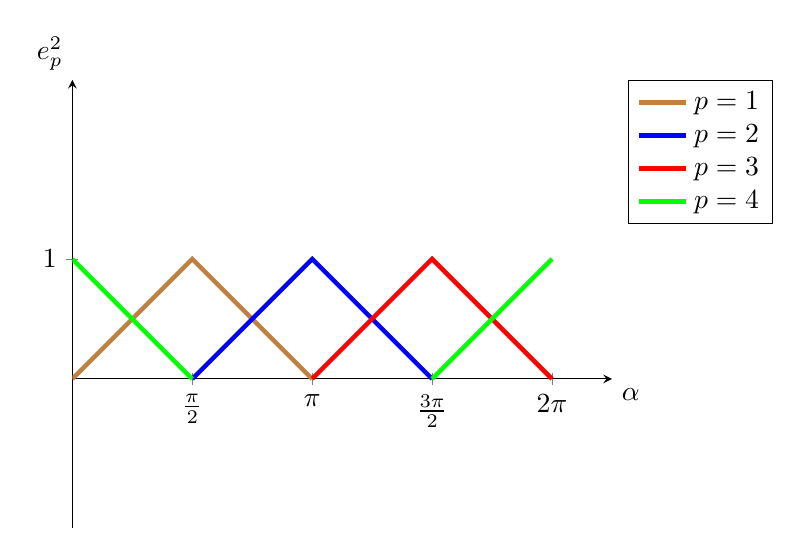
\begin{tikzpicture}
  \begin{axis}[xmax=4.5,
               xmin=0,
               ymin=0,
               ymax=1.25,
               xlabel={$\alpha$},
               ylabel={$e_p^2$},
               xtick={1, 2, 3, 4},
               xticklabels={$\frac{\pi}{2}$, $\pi$, $\frac{3\pi}{2}$, $2\pi$},
               ytick={1},
               axis equal,
               axis x line=center,
               axis y line=center,
               xlabel style={below right},
               ylabel style={above left},
               legend pos=outer north east]
    \addplot [ultra thick, brown] coordinates {(0,0)(1,1)(2,0)};
    \addlegendentry{$p = 1$}
    \addplot [ultra thick, blue] coordinates {(1,0)(2,1)(3,0)};
    \addlegendentry{$p = 2$}
    \addplot [ultra thick, red] coordinates {(2,0)(3,1)(4,0)};
    \addlegendentry{$p = 3$}
    \addplot [ultra thick, green] coordinates {(3,0)(4,1)};
    \addlegendentry{$p = 4$}
    \addplot [ultra thick, green] coordinates {(0,1)(1,0)};
  \end{axis}
\end{tikzpicture}
\end{center}


\subsubsection{Effiziente Berechnung für $K=2$}

Wir können für $K=2$ die Basis-Berechnung durch
\begin{equation}
  e_p^2\left(\alpha\right) = \begin{cases}
    \min\left(\frac{P}{2\pi} \alpha - p + 1, 0\right), & \text{wenn }\alpha \leq t\left(p\right)\text{,}\\
    \min\left(-\frac{P}{2\pi} \alpha + p + 1, 0\right), & \text{sonst}
  \end{cases}
\end{equation}
vereinfachen.

\begin{proof}
  Aufsteigende Gerade der Dreiecksfunktion für $p$, $1 \leq p \leq P$, ist definiert durch
  \begin{equation}
    \frac{\alpha - t\left(p-1\right)}{t\left(p\right) - t\left(p-1\right)} = \frac{P\left(\alpha - t\left(p-1\right)\right)}{2\pi} = \frac{P\alpha - 2\pi\left(p-1\right)}{2\pi} = \frac{P}{2\pi}\alpha - p + 1.
  \end{equation}
  $\min \left(\frac{P}{2\pi} \alpha - p + 1, 0\right)$ beschreibt damit die linke Seite des Dreiecks.
  Analog für absteigende Gerade.
\end{proof}

Die Fallunterscheidung ist unnötig, wir können uns einfach immer für das Minimum der beiden entscheiden.
Die Grafik zeigt dies ziemlich eindeutig.
Das ergibt letztendlich
\begin{equation}
  e_p^2\left(\alpha\right) = \min \left( \min\left(\frac{P}{2\pi} \alpha - p + 1, 0\right), \min\left(-\frac{P}{2\pi} \alpha + p + 1, 0\right) \right)\text{.}
\end{equation}

\begin{figure}
  \centering
  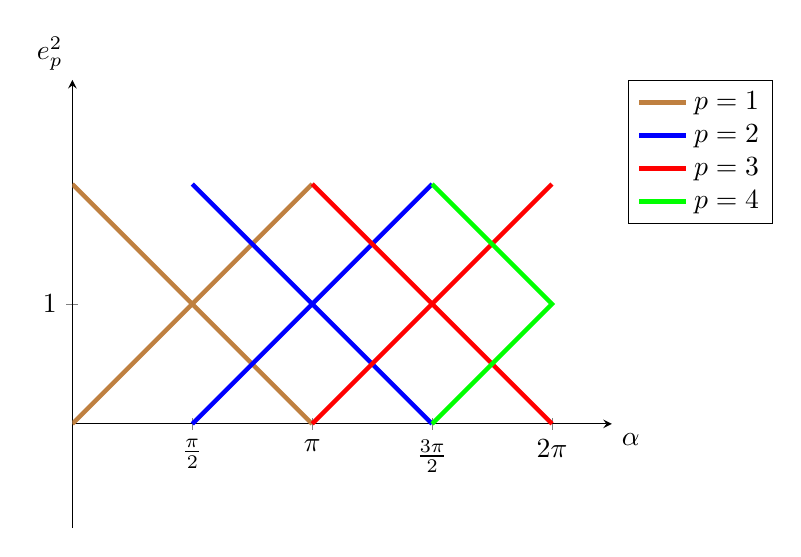
\begin{tikzpicture}
    \begin{axis}[xmax=4.5,
                 xmin=0,
                 ymin=0,
                 ymax=2,
                 xlabel={$\alpha$},
                 ylabel={$e_p^2$},
                 xtick={1, 2, 3, 4},
                 xticklabels={$\frac{\pi}{2}$, $\pi$, $\frac{3\pi}{2}$, $2\pi$},
                 ytick={1},
                 axis equal,
                 axis x line=center,
                 axis y line=center,
                 xlabel style={below right},
                 ylabel style={above left},
                 legend pos=outer north east]
      \addplot [ultra thick, brown] coordinates {(0,0)(2,2)(1,1)(0,2)(2,0)};
      \addlegendentry{$p = 1$}
      \addplot [ultra thick, blue] coordinates {(1,0)(3,2)(2,1)(1,2)(3,0)};
      \addlegendentry{$p = 2$}
      \addplot [ultra thick, red] coordinates {(2,0)(4,2)(3,1)(2,2)(4,0)};
      \addlegendentry{$p = 3$}
      \addplot [ultra thick, green] coordinates {(3,0)(4,1)(3,2)};
      \addlegendentry{$p = 4$}
    \end{axis}
  \end{tikzpicture}
\end{figure}


Wir haben bisher noch nicht den \emph{Kreis} geschlossen mit unserer Formel.

Das können wir aber leicht tun, indem wir unsere absteigenden Geraden um $2\pi$ nach links verschieben und daraus wiederum das Minimum von $0$ ziehen.
Dann sind diese Geraden außer für $p = P$ im Gültigkeitsbereich der Funktion allesamt $0$.
Wir können demnach aus unserer bisherigen Formel und der verschobenen Gerade das Maximum ziehen.
Wir erhalten
\begin{equation}
\begin{split}
  e_p^2\left(\alpha\right) = \max \biggr( & \min \left( \min\left(\frac{P}{2\pi} \alpha - p + 1, 0\right), \min\left(-\frac{P}{2\pi} \alpha + p + 1, 0\right) \right),\\
  & \min \left(-\frac{P}{2\pi} \left( \alpha + 2\pi \right) + p + 1, 0\right) \biggr)\text{.}
\end{split}
\end{equation}

\subsection{Tensorimplementierung}

\begin{equation}
\begin{split}
  \gls{Fout} = & \ {\left(\gls{Adistnorm}\right)}_{ii} \cdot \gls{F} \cdot \ma{W}_{P+1}\\
  & + \sum_{p=1}^P \gls{Adistnorm} \gls{hadamard} e^K_p\left(\gls{Arad}\right) \cdot \gls{F} \cdot \ma{W}_{p}
\end{split}
\end{equation}

\gls{Adistnorm} enthält einmal nur die Diagonale und einmal alles ohne Diagonale.

\newpage


\subsection{Grundlagen}

\begin{itemize}
  \item ungerichtete Distanzadjazenzmatrix $\gls{Adist} \in \gls{R+}^{N \times N} = {\left(a\right)}_{ij}$
  \item (lokal) normalisierte ungerichtete Distanzadjazenzmatrix $\gls{Adistnorm} \in \gls{R+}^{N \times N} = {\left(\tilde a\right)}_{ij}$
  \item gerichtete Winkeladjazenzmatrix $\gls{Arad} \in \gls{R+}^{N \times N} = {\left(\alpha\right)}_{ij}$
  \item Input-Featurematrix $\gls{F} \in \gls{R}^{N \times X} = {\left(f\right)}_{ij}$
  \item Output-Featurematrix $\gls{Fout} \in \gls{R}^{N \times Y} = {\left(f^{\prime}\right)}_{ij}$
  \item Anzahl Partitionen $P \in \gls{N}$
  \item Gewichtstensor $\ma{W} \in \gls{R}^{\left(P + 1\right) \times X \times Y} = {\left(w\right)}_{ijw}$
\end{itemize}

\subsection{Faltung}

\begin{equation}
  f^{\prime}_{iy} = \sum_{x = 1}^X \tilde a_{ii} \cdot f_{ix} \cdot w_{\left(P +1\right)xy} \sum_{n = 1, n \neq i}^N \tilde a_{in} \cdot f_{nx} \cdot b^K_P\left(\alpha_{in}, x, y\right)
\end{equation}
wobei $b_P^K$ eine B-Spline-Kurve.

Es ist anzumerken, dass im Summanden der betrachtete Knoten übersprungen wird, da für diesen ein Wert in der Winkelmatrix keinen Sinn ergibt.
Er wird daher in der Faltung jeweils einzeln mit einem Gewicht multipliziert und dazuaddiert.

\subsection{B-Spline-Kurven}

$b_P^K \colon \left]0, 2\pi\right] \times \left\{1, \ldots, X \right\} \times \left\{1, \ldots, Y\right\} \to \gls{R}$ ist eine B-Spline-Kurve der Ordnung $K \in \gls{N}$ auf den Kantenwinkeln des Graphen.
Bemerke, dass wir $0$ für Winkel aussschließen und stattdessen den Winkel $2\pi$ benutzen, so dass wir nicht mit der Bedeutung von $0$ bei Adjazenzmatrizen in die Quere kommen.
\begin{equation}
  b_P^K\left(\alpha, x, y \right) = \sum_{p=1}^P w_{pxy} \cdot e_p^K\left(\alpha\right)
\end{equation}
wobei die Basisfunktion $e_p^K$ rekursiv über $K$ definiert ist mit Initialisierung
\begin{equation}
  e_p^1\left(\alpha\right) = \begin{cases}
    1, & \text{wenn }\alpha \in \left] t\left(p-1\right), t\left(p\right)\right]\text{,}\\
    0, & \text{sonst}
  \end{cases}
\end{equation}
und Rekursionsschritt
\begin{equation}
  e_p^k\left(\alpha\right) = \frac{\alpha - t\left(p - 1\right)}{t\left(p+k-2\right) - t\left(p - 1\right)} e_p^{k-1}\left(\alpha\right) + \frac{t\left(i\left(p + k - 1\right)\right) - \alpha}{t\left(p+k - 1\right) - t\left(p\right)} e_{i\left(p+1\right)}^{k-1}\left(\alpha\right)
\end{equation}
wobei $t \colon \gls{N} \to \gls{R}$ mit $t\left(p\right) = 2\pi\frac{p}{P}$ und $i\left(p\right) = \gls{modulo}\left(p-1, P\right) + 1$.
Es ist anzumerken, dass wir $t$ und $i$ dabei für den Rekursionsschritt über die Grenze $P$ hinaus definieren.
Das hilft uns, die B-Spline-Kurve \emph{kreisförmig} abzuschließen.

Je größer $K$ gesetzt wird, umso mehr Anteile anderer benachbarter Stützpunkte fließen in die Berechnung mit ein.
Die Größe von $K$ wird deshalb auch oft \emph{lokale Kontrollierbarkeit} genannt.

\subsubsection{Beispiel mit $P=4$}

\begin{center}
\begin{tikzpicture}
  \begin{axis}[xmax=4.5,
               xmin=0,
               ymin=0,
               ymax=1.25,
               xlabel={$\alpha$},
               ylabel={$e_p^1$},
               xtick={1, 2, 3, 4},
               xticklabels={$\frac{\pi}{2}$, $\pi$, $\frac{3\pi}{2}$, $2\pi$},
               ytick={1},
               axis equal,
               axis x line=center,
               axis y line=center,
               xlabel style={below right},
               ylabel style={above left},
               legend pos=outer north east]
    \addplot [ultra thick, brown] coordinates {(0,1)(1,1)};
    \addlegendentry{$p = 1$}
    \addplot [ultra thick, blue] coordinates {(1,1)(2,1)};
    \addlegendentry{$p = 2$}
    \addplot [ultra thick, red] coordinates {(2,1)(3,1)};
    \addlegendentry{$p = 3$}
    \addplot [ultra thick, green] coordinates {(3,1)(4,1)};
    \addlegendentry{$p = 4$}
  \end{axis}
\end{tikzpicture}
\end{center}

\begin{center}
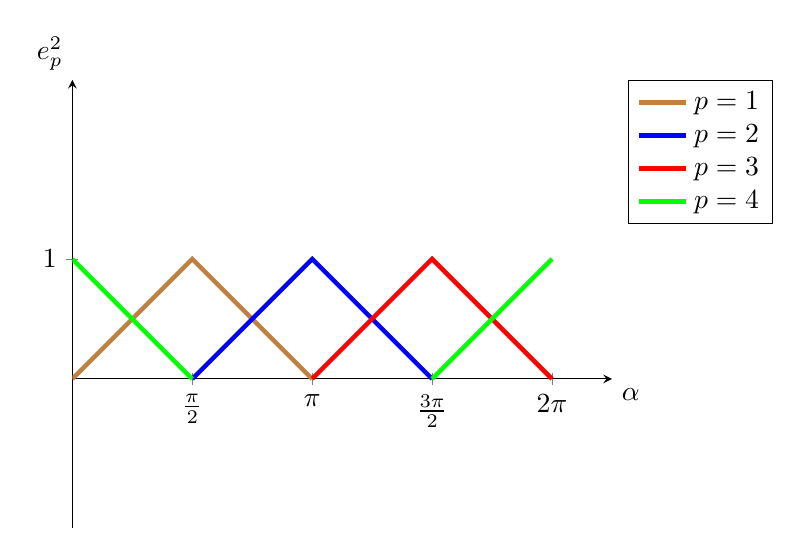
\begin{tikzpicture}
  \begin{axis}[xmax=4.5,
               xmin=0,
               ymin=0,
               ymax=1.25,
               xlabel={$\alpha$},
               ylabel={$e_p^2$},
               xtick={1, 2, 3, 4},
               xticklabels={$\frac{\pi}{2}$, $\pi$, $\frac{3\pi}{2}$, $2\pi$},
               ytick={1},
               axis equal,
               axis x line=center,
               axis y line=center,
               xlabel style={below right},
               ylabel style={above left},
               legend pos=outer north east]
    \addplot [ultra thick, brown] coordinates {(0,0)(1,1)(2,0)};
    \addlegendentry{$p = 1$}
    \addplot [ultra thick, blue] coordinates {(1,0)(2,1)(3,0)};
    \addlegendentry{$p = 2$}
    \addplot [ultra thick, red] coordinates {(2,0)(3,1)(4,0)};
    \addlegendentry{$p = 3$}
    \addplot [ultra thick, green] coordinates {(3,0)(4,1)};
    \addlegendentry{$p = 4$}
    \addplot [ultra thick, green] coordinates {(0,1)(1,0)};
  \end{axis}
\end{tikzpicture}
\end{center}


\subsubsection{Effiziente Berechnung für $K=2$}

Wir können für $K=2$ die Basis-Berechnung durch
\begin{equation}
  e_p^2\left(\alpha\right) = \begin{cases}
    \min\left(\frac{P}{2\pi} \alpha - p + 1, 0\right), & \text{wenn }\alpha \leq t\left(p\right)\text{,}\\
    \min\left(-\frac{P}{2\pi} \alpha + p + 1, 0\right), & \text{sonst}
  \end{cases}
\end{equation}
vereinfachen.

\begin{proof}
  Aufsteigende Gerade der Dreiecksfunktion für $p$, $1 \leq p \leq P$, ist definiert durch
  \begin{equation}
    \frac{\alpha - t\left(p-1\right)}{t\left(p\right) - t\left(p-1\right)} = \frac{P\left(\alpha - t\left(p-1\right)\right)}{2\pi} = \frac{P\alpha - 2\pi\left(p-1\right)}{2\pi} = \frac{P}{2\pi}\alpha - p + 1.
  \end{equation}
  $\min \left(\frac{P}{2\pi} \alpha - p + 1, 0\right)$ beschreibt damit die linke Seite des Dreiecks.
  Analog für absteigende Gerade.
\end{proof}

Die Fallunterscheidung ist unnötig, wir können uns einfach immer für das Minimum der beiden entscheiden.
Die Grafik zeigt dies ziemlich eindeutig.
Das ergibt letztendlich
\begin{equation}
  e_p^2\left(\alpha\right) = \min \left( \min\left(\frac{P}{2\pi} \alpha - p + 1, 0\right), \min\left(-\frac{P}{2\pi} \alpha + p + 1, 0\right) \right)\text{.}
\end{equation}

\begin{figure}
  \centering
  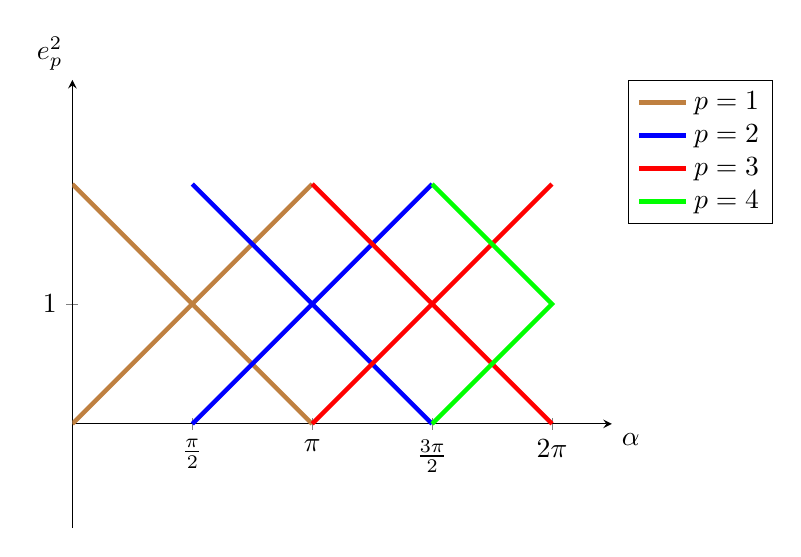
\begin{tikzpicture}
    \begin{axis}[xmax=4.5,
                 xmin=0,
                 ymin=0,
                 ymax=2,
                 xlabel={$\alpha$},
                 ylabel={$e_p^2$},
                 xtick={1, 2, 3, 4},
                 xticklabels={$\frac{\pi}{2}$, $\pi$, $\frac{3\pi}{2}$, $2\pi$},
                 ytick={1},
                 axis equal,
                 axis x line=center,
                 axis y line=center,
                 xlabel style={below right},
                 ylabel style={above left},
                 legend pos=outer north east]
      \addplot [ultra thick, brown] coordinates {(0,0)(2,2)(1,1)(0,2)(2,0)};
      \addlegendentry{$p = 1$}
      \addplot [ultra thick, blue] coordinates {(1,0)(3,2)(2,1)(1,2)(3,0)};
      \addlegendentry{$p = 2$}
      \addplot [ultra thick, red] coordinates {(2,0)(4,2)(3,1)(2,2)(4,0)};
      \addlegendentry{$p = 3$}
      \addplot [ultra thick, green] coordinates {(3,0)(4,1)(3,2)};
      \addlegendentry{$p = 4$}
    \end{axis}
  \end{tikzpicture}
\end{figure}


Wir haben bisher noch nicht den \emph{Kreis} geschlossen mit unserer Formel.

Das können wir aber leicht tun, indem wir unsere absteigenden Geraden um $2\pi$ nach links verschieben und daraus wiederum das Minimum von $0$ ziehen.
Dann sind diese Geraden außer für $p = P$ im Gültigkeitsbereich der Funktion allesamt $0$.
Wir können demnach aus unserer bisherigen Formel und der verschobenen Gerade das Maximum ziehen.
Wir erhalten
\begin{equation}
\begin{split}
  e_p^2\left(\alpha\right) = \max \biggr( & \min \left( \min\left(\frac{P}{2\pi} \alpha - p + 1, 0\right), \min\left(-\frac{P}{2\pi} \alpha + p + 1, 0\right) \right),\\
  & \min \left(-\frac{P}{2\pi} \left( \alpha + 2\pi \right) + p + 1, 0\right) \biggr)\text{.}
\end{split}
\end{equation}

\subsection{Tensorimplementierung}

\begin{equation}
\begin{split}
  \gls{Fout} = & \ {\left(\gls{Adistnorm}\right)}_{ii} \cdot \gls{F} \cdot \ma{W}_{P+1}\\
  & + \sum_{p=1}^P \gls{Adistnorm} \gls{hadamard} e^K_p\left(\gls{Arad}\right) \cdot \gls{F} \cdot \ma{W}_{p}
\end{split}
\end{equation}

\gls{Adistnorm} enthält einmal nur die Diagonale und einmal alles ohne Diagonale.

\newpage


Sei \gls{G} ein Graph im zweidimensionalen euklidschen Raum, eindeutig definiert über $\gls{Adist} \in {\left[0, 1\right)}^{N \times N}$ und $\gls{Arad} \in {\left[0, 2\pi\right]}^{N \times N}$.
Dann lässt sich \gls{G} in $P \in \gls{N}$ Bereiche ${\left\{\gls{A}_p\right\}}_{p=1}^P$ \emph{partitionieren}, sodass
\begin{equation}
  {\left(\gls{A}_p\right)}_{ij} \coloneqq \begin{cases}
    {\left(\gls{Adist}\right)}_{ij}, & \text{wenn } {\left(\gls{Arad}\right)}_{ij} \in \left(\frac{2\pi}{P}\left(p-1\right), \frac{2\pi}{P}p\right]\\
    0, & \text{sonst.}
  \end{cases}
  \label{eq:partitionierung}
\end{equation}
Damit beschreiben die Matrizen ${\left\{\gls{A}_p\right\}}_{p=1}^P$ disjunkte Partitionen der Kanten des Graphen \gls{G} abhängig von ihren Ausrichtungen im Raum mit $\gls{Adist} = \sum_{p=1}^P \gls{A}_p$.
$\gls{A}_p$ ist insbesondere nicht zwingend symmetrisch, da ${\left(\gls{Arad}\right)}_{ij} \neq {\left(\gls{Arad}\right)}_{ji}$ für alle $\gls{v}_i, \gls{v}_j \in \gls{V}$ mit $\gls{v}_j \in \gls{Neighbor}\left(\gls{v}_i\right)$.
Abbildung~\ref{fig:partitionierung} veranschaulicht den Prozess der Partitionierung.
Mit $P = 8$ erhalten die jeweiligen Bereiche einen gleichmäßigen Innenwinkel von $\pi/4$.

Es lässt sich analog zu Kapitel~\ref{graph_convolutional_networks} ein Faltungsoperator definieren, bei dem nun aber jeder Partition ein eigener frei trainierbarer Parameter zugeordnet wird.
Der Parameter einer Partition hat damit folglich eine eindeutige Örtlichkeitszuweisung über das Intervall \bzw{} den Bereich der Richtungen seiner Kanten.
Analog zu~\eqref{eq:gcn_renorm} muss dafür zuerst die (Re-)normalisierung der Form
\begin{equation*}
  \gls{Ddisttilde}^{-\frac{1}{2}}\gls{Adisttilde}\gls{Ddisttilde}^{-\frac{1}{2}} = \gls{Ddisttilde}^{-1} + \sum_{p=1}^P \gls{Ddisttilde}^{-\frac{1}{2}}\gls{A}_p\gls{Ddisttilde}^{-\frac{1}{2}}
\end{equation*}
mit $\gls{Adisttilde} \coloneqq \gls{Adist} + \gls{I}$ und ${\left(\gls{Ddisttilde}\right)}_{ii} \coloneqq \sum_{j=1}^N {\left(\gls{Adisttilde}\right)}_{ij}$ durchgeführt werden.
Dies lässt sich mit Hilfe von $\gls{Adist} = \sum_{p=1}^P \gls{A}_p$ und $\gls{Ddisttilde}^{-1/2}\gls{Ddisttilde}^{-1/2} = \gls{Ddisttilde}^{-1}$ verifizieren.
Im Folgenden sei $\gls{Atilde}_p \coloneqq \gls{Ddisttilde}^{-1/2}\gls{A}_p\gls{Ddisttilde}^{-1/2}$ für $p \in \left\{1, \ldots, P \right\}$ und $\gls{Atilde}_0 \coloneqq \gls{Ddisttilde}^{-1}$.
Dann folgt sofort für den Faltungsoperatur $\ve{f}_{\mathrm{in}} \star \ve{\hat g}$ auf Graphen im zweidimensionalen euklidschen Raum, dass dieser
\begin{equation}
  \ve{f}_{\mathrm{in}} \star \ve{\hat g} \approx \sum_{p=0}^P c_p \gls{Atilde}_p \ve{f}_{\mathrm{in}}
\end{equation}
mit den freien Parametern $c_0, \ldots, c_P \in \gls{R}$ erfüllt.

Es stellt sich heraus, dass die Faltung auf den Partitionierungen eines regulären Gittergraphen mit $P=8$ äquivalent zu der klassischen Faltung auf einem regulären Gitter mit Filtergröße $3 \times 3$ ist.
\begin{proof}
  Sei \gls{G} ein (unendlicher) regulärer Gittergraph mit Konnektivität $8$ bei Kantengewichten $\exp\left(-1/\gls{sigma}^2\right)$ respektive $\exp\left(-2/\gls{sigma}^2\right)$, $\gls{W} \in \gls{R}^{3 \times 3}$ Filtermatrix der klassischen Faltung und $\ve{f}_{\mathrm{in}}$ Merkmalsvektor auf dem Graphen mit Koordinatenindexnotation ${\left(\ve{f}_{\mathrm{in}}\right)}_{x,y}$.
  Die klassische Faltung an einem Gitterpunkt $\left(x, y\right)$ ist dann gegeben als
  \begin{equation}
    {\left(\ve{f}_{\mathrm{out}}\right)}_{x,y} = \sum_{i,j \in \left\{1, 2, 3\right\}} {\left(\ve{f}_{\mathrm{in}}\right)}_{x+i-2, y+j-2} \gls{W}_{i, j}
  \end{equation}
  $\gls{Atilde}_p$ besitzt aufgrund von $P = 8$ genau einen Eintrag pro Matrixreihe.



  % $\gls{v}_{x,y}$ ein Knoten in \gls{G}. Mit $\gls{Atilde}_0 = \gls{Ddisttilde}^{-1}$ folgt, dass ${\left(\ve{f}_{\mathrm{out}}\right)}_{x,y} = $
\end{proof}

Obwohl
Eine Lösung zu diesem Problem ist die Interpolation der Innenwinkel über die Basisfunktionen einer B-Spline-Kurve.

% \begin{equation}
%   f^{\prime}_{iy} = \sum_{x = 1}^X \tilde a_{ii} \cdot f_{ix} \cdot w_{\left(P +1\right)xy} \sum_{n = 1, n \neq i}^N \tilde a_{in} \cdot f_{nx} \cdot b^K_P\left(\alpha_{in}, x, y\right)
% \end{equation}
% wobei $b_P^K$ eine B-Spline-Kurve.
% \todo{$a_{ii}$ kann raus, da immer $1$}

% Es ist anzumerken, dass im Summanden der betrachtete Knoten übersprungen wird, da für diesen ein Wert in der Winkelmatrix keinen Sinn ergibt.
% Er wird daher in der Faltung jeweils einzeln mit einem Gewicht multipliziert und dazuaddiert.

% \paragraph{B-Spline-Kurven}
% \label{bspline}

% $b_P^K \colon \left(0, 2\pi\right]\to\gls{R}$ ist eine \emph{B-Spline-Kurve} der Ordnung $K \in \gls{N}$ mit $P \in \gls{N}$ Kontrollpunkten auf den Kantenwinkeln $\left(0, 2\pi\right]$ eines Graphknotens $\gls{v}_i$ zu seinen adjazenten Knoten $\gls{v}_j$.
% Es ist wichtig anzumerken, dass Null für Winkel ausgeschlossen werden und stattdessen der Winkel $2\pi$ benutzt wird, so dass wir nicht mit der Bedeutung von $0$ in Adjazenzmatrizen in die Quere kommen.
% \\\\
% \begin{equation}
%   b_P^K\left(\alpha, x, y \right) = \sum_{p=1}^P w_{pxy} \cdot e_p^K\left(\alpha\right)
% \end{equation}
% wobei die Basisfunktion $e_p^K$ rekursiv über $K$ definiert ist mit Initialisierung
% \begin{equation}
%   e_p^1\left(\alpha\right) = \begin{cases}
%     1, & \text{wenn }\alpha \in \left] t\left(p-1\right), t\left(p\right)\right]\text{,}\\
%     0, & \text{sonst}
%   \end{cases}
% \end{equation}
% und Rekursionsschritt
% \begin{equation}
%   e_p^k\left(\alpha\right) = \frac{\alpha - t\left(p - 1\right)}{t\left(p+k-2\right) - t\left(p - 1\right)} e_p^{k-1}\left(\alpha\right) + \frac{t\left(i\left(p + k - 1\right)\right) - \alpha}{t\left(p+k - 1\right) - t\left(p\right)} e_{i\left(p+1\right)}^{k-1}\left(\alpha\right)
% \end{equation}
% wobei $t \colon \gls{N} \to \gls{R}$ mit $t\left(p\right) = 2\pi\frac{p}{P}$ und $i\left(p\right) = \gls{modulo}\left(p-1, P\right) + 1$.
% Es ist anzumerken, dass wir $t$ und $i$ dabei für den Rekursionsschritt über die Grenze $P$ hinaus definieren.
% Das hilft uns, die B-Spline-Kurve \emph{kreisförmig} abzuschließen.

% Je größer $K$ gesetzt wird, umso mehr Anteile anderer benachbarter Stützpunkte fließen in die Berechnung mit ein.
% Die Größe von $K$ wird deshalb auch oft \emph{lokale Kontrollierbarkeit} genannt.

% \paragraph{Faltungsoperator}
% \label{ebener_faltungsoperator}
